\documentclass{article}
\usepackage{graphicx}
\usepackage{booktabs}
\usepackage{longtable,tabu}
\usepackage{listings}
\usepackage{hyperref}
\title{SA Calibration }
%\author
\begin{document}
\maketitle
\section{Section 1}


Some results from the calibration done using Weights and Biases for South Africa Model before changing covasim model code. \\ 

The following calibration graphs are obtained using observed data from Gauteng. The first graph shows the likelihood for each sweep. The change evident in the graph is after interrupting the sweeps by changing the set of observed data used to calculate likelihood and simulation dates (i.e removed data form 5 March to 14 May 2020. During this period number of cumulative infections were less than 100 and local transmission was very low). Calibration was based on 5 parameters - beta, pop\_infected, rel\_crit\_prob, rel\_death\_prob and rel\_severe\_prob. The best sweep had likelihood = -4075.452. Total population is 15 million using a scale factor of 1:10. 

\begin{figure}[ht]
	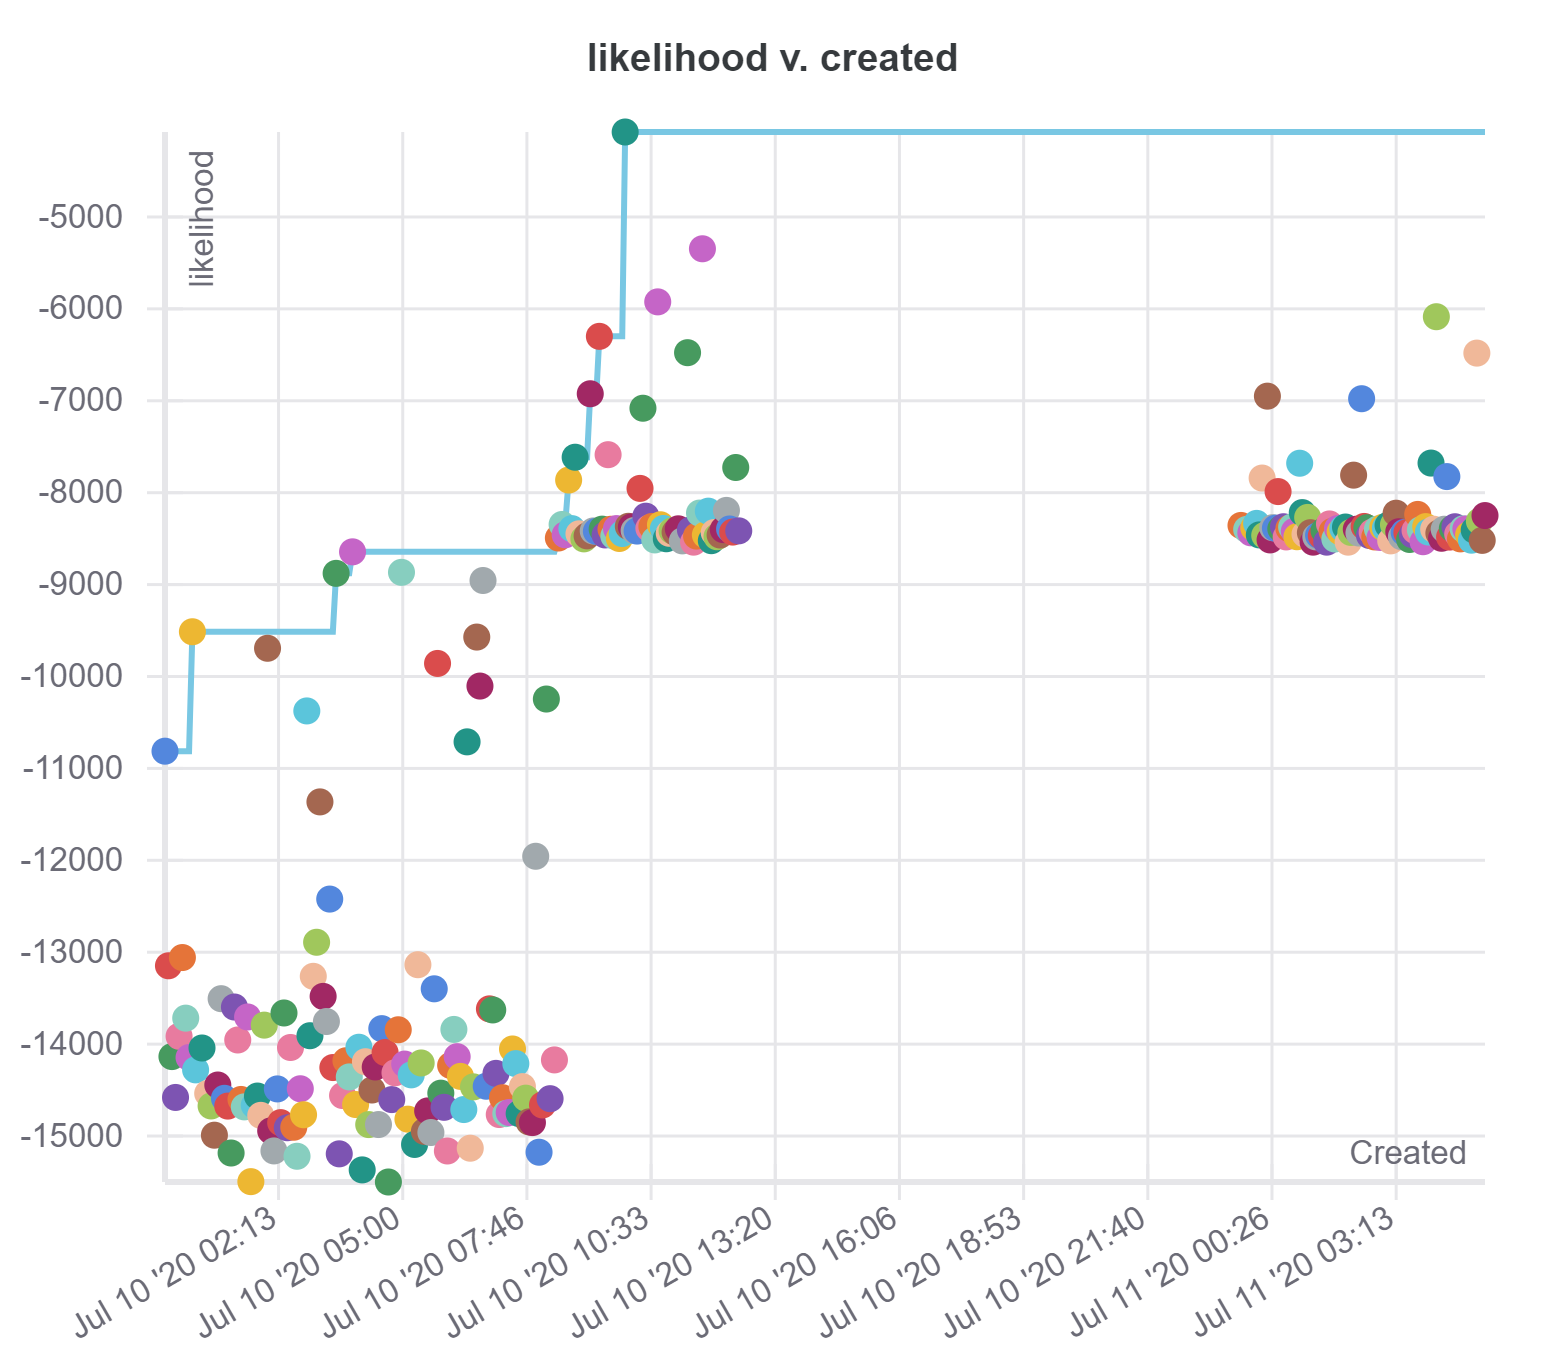
\includegraphics[width=0.5\linewidth]{charts/Section-1-Panel-0-unp6o2mj4}
	\includegraphics[width=0.5\linewidth]{charts/Section-1-Panel-2-oya2j7xix}
\end{figure} 


The following graphs were obtained using total population of 15 million and a scale factor of 1:10 and cumulative infection data from 23 May 2020 to 8 July 2020 (excluding number of deaths). Best sweep had likelihood = -1732.896.    

\begin{figure}[ht]
	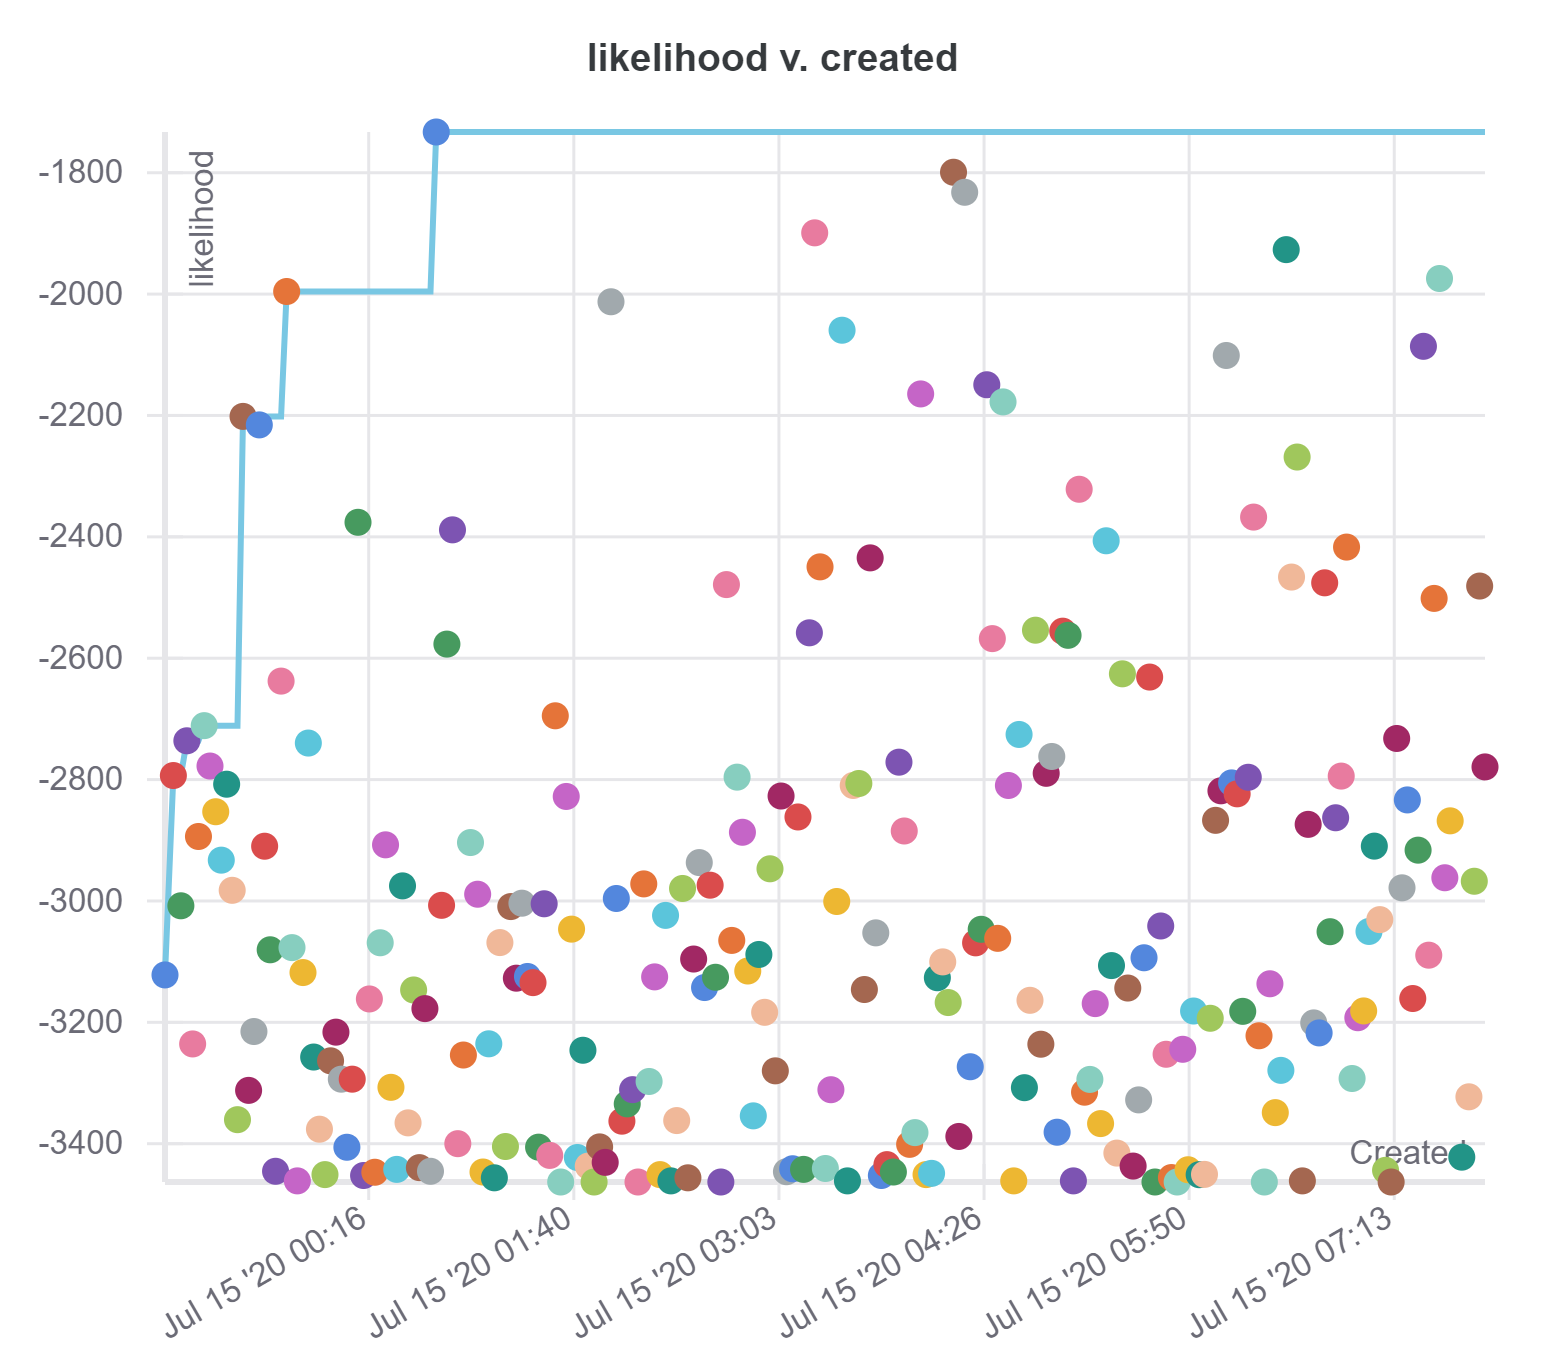
\includegraphics[width=0.5\linewidth]{charts/Section-1-Panel-2-469nwslew}
	\includegraphics[width=0.5\linewidth]{charts/Section-1-Panel-4-z2mgng6y1}
\end{figure}

\newpage
Graph showing simulation data superimposed on observed data for the best sweep is as follows: 
\begin{figure}[ht]
	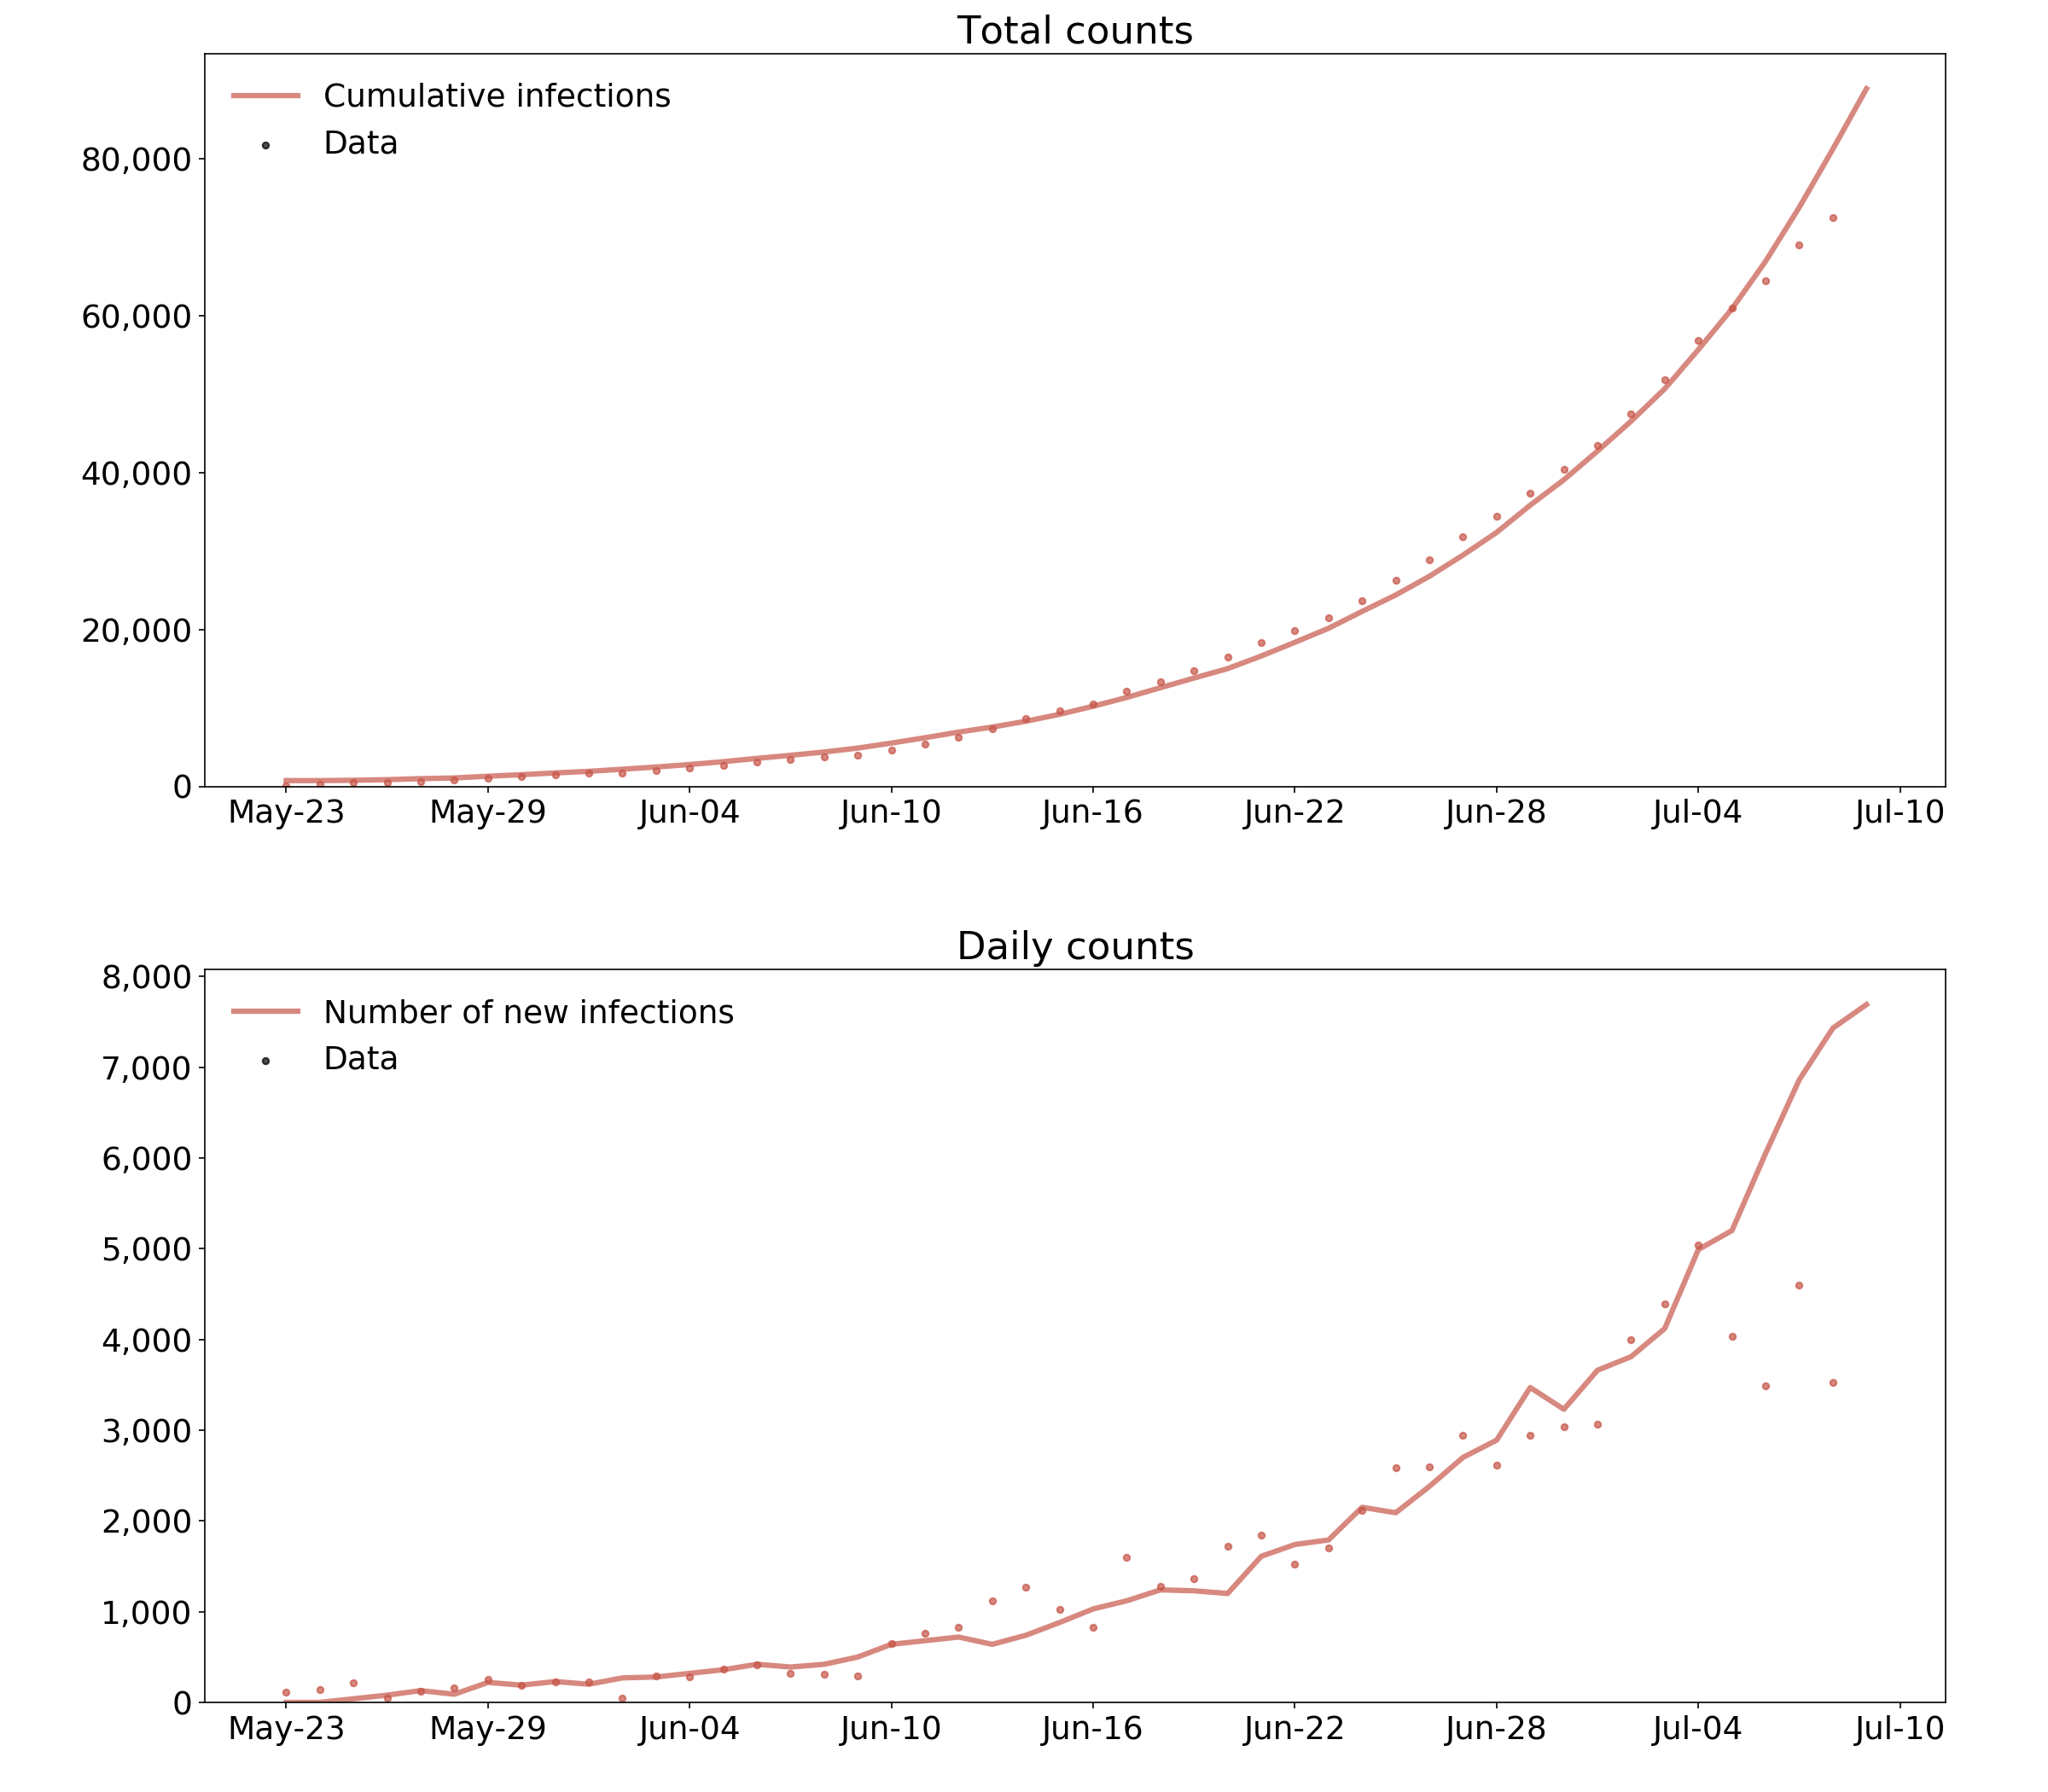
\includegraphics[width=0.5\linewidth]{charts/Best_fit}
\end{figure}

Graphs obtained using total population of 15 million and a scale factor of 1:10,  cumulative infection data and cummulative deaths from 23 May 2020 to 8 July 2020 are as follows: \\    
\begin{figure}[ht]
	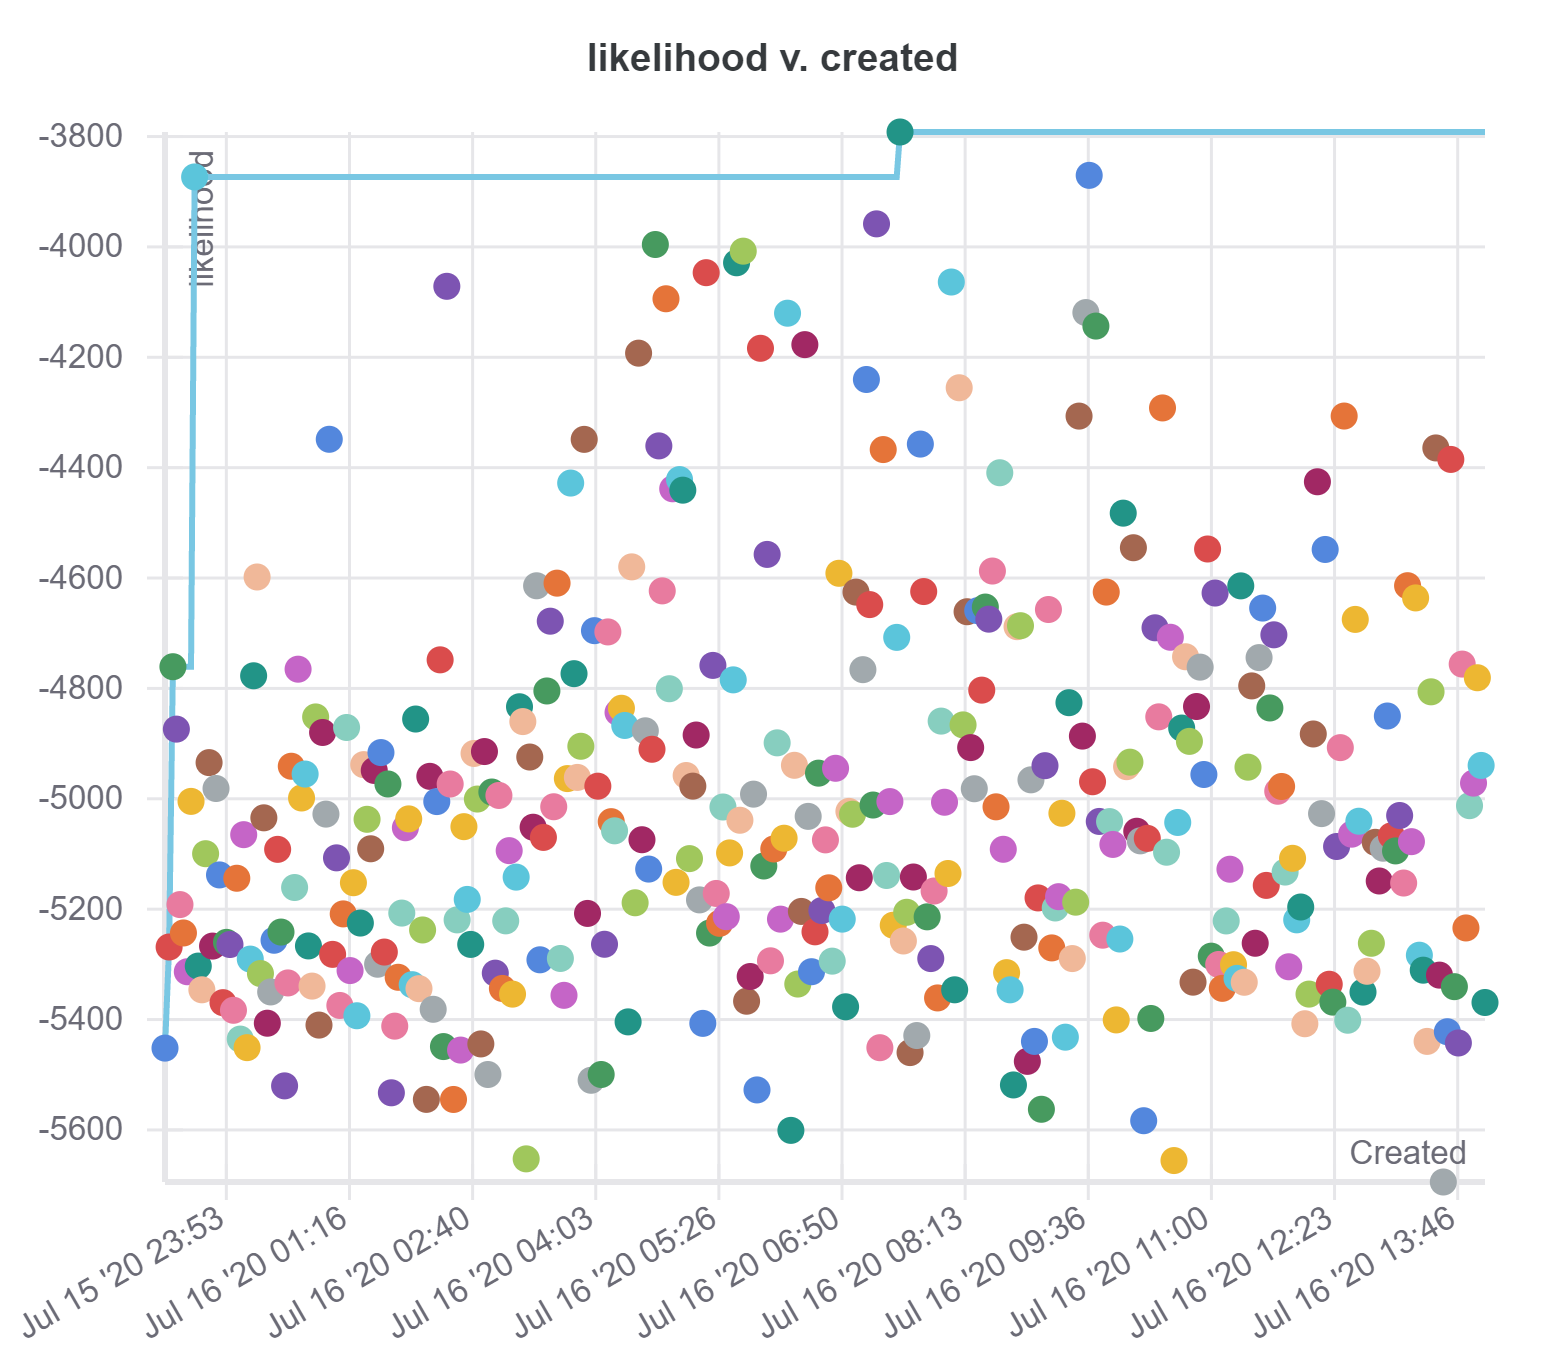
\includegraphics[width=0.5\linewidth]{charts/Section-1-Panel-0-90491c2ri}
	\includegraphics[width=0.5\linewidth]{charts/Section-1-Panel-2-aprnkodlm}
\end{figure}

Graph showing simulation data superimposed on observed data for the best sweep is as follows: 
\begin{figure}[ht]
	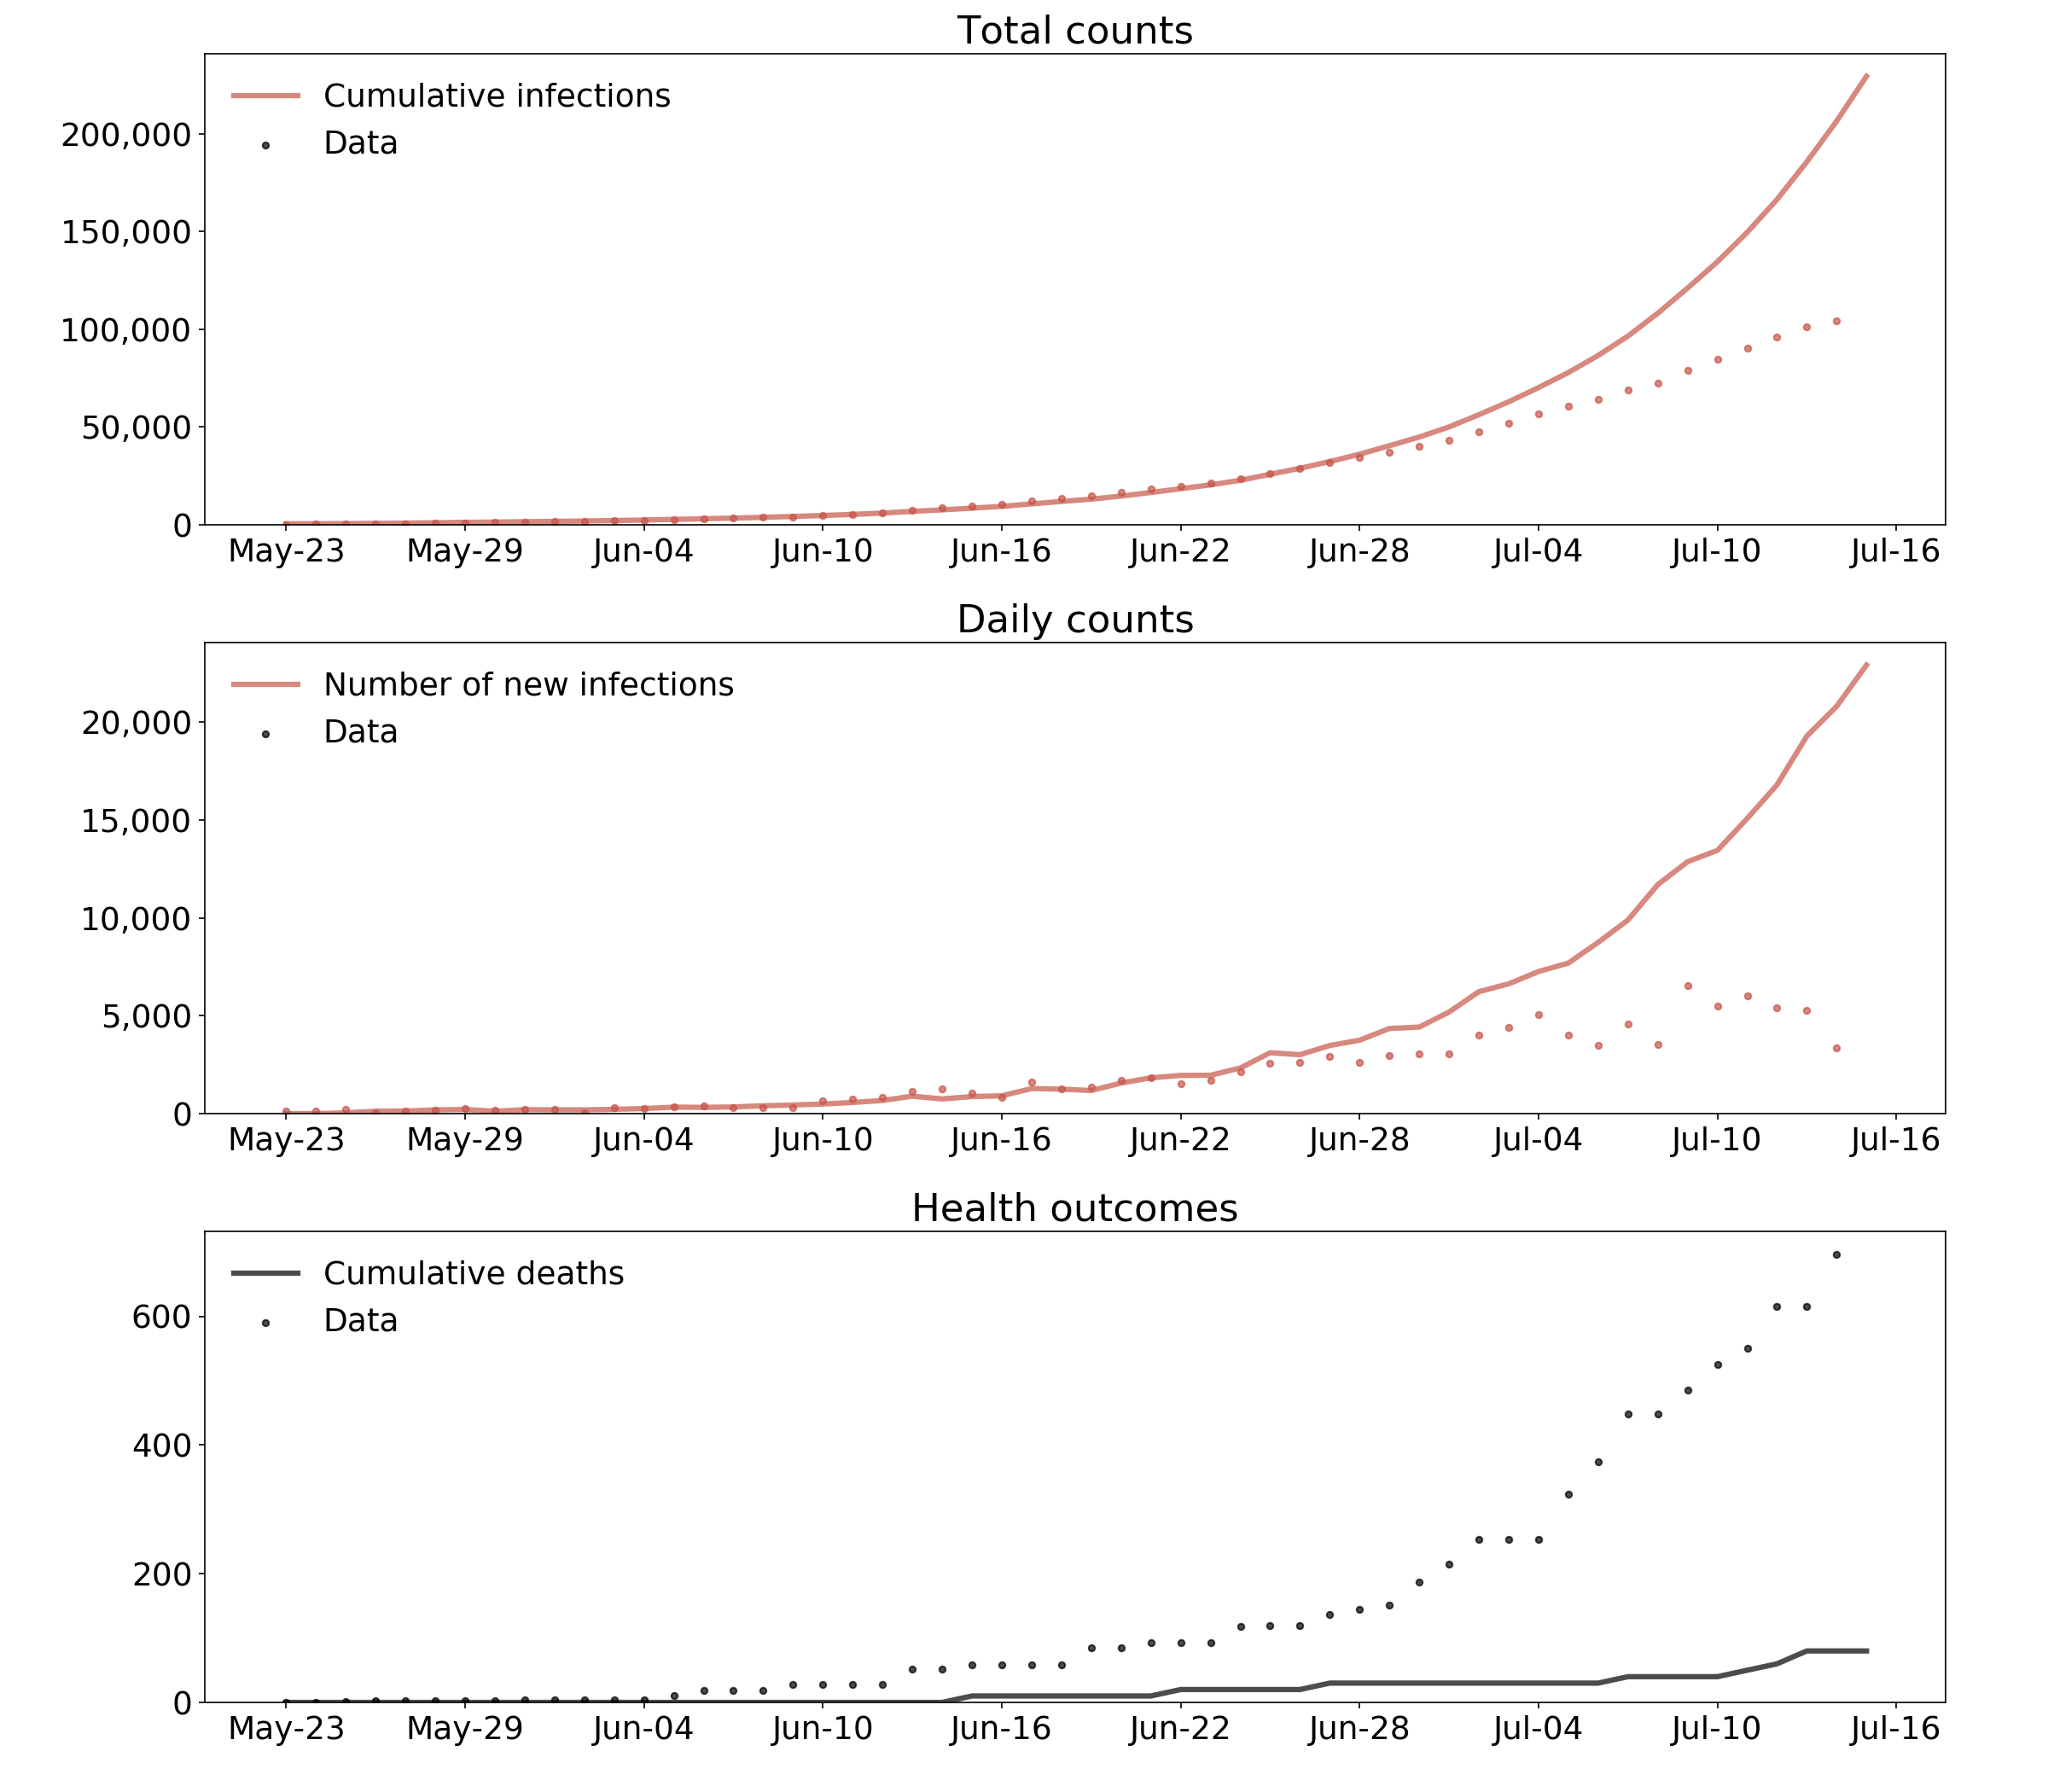
\includegraphics[width=0.5\linewidth]{charts/Best_fit2}
\end{figure}



\newpage
\begin{thebibliography}{9}
\bibitem{wandb}
  Weights and Biases,
  \href{https://app.wandb.ai/mudimu/covasim/reports/SA-Calibration---VmlldzoyMDQ0MDk}{https://wandb.com}
\end{thebibliography}
\end{document}